\documentclass[12pt]{jreport}
\usepackage[dvipdfmx]{graphicx}

%\usepackage[bachelor]{AIcover}	% 卒論の場合
\usepackage[master]{AIcover}		% 修論の場合

\usepackage{AIthesis}
\usepackage{geometry}

\input personal

\begin{document}
\makeCoverPageII
\newpage

\newgeometry{margin=0mm}
\begin{figure}
  \centering
  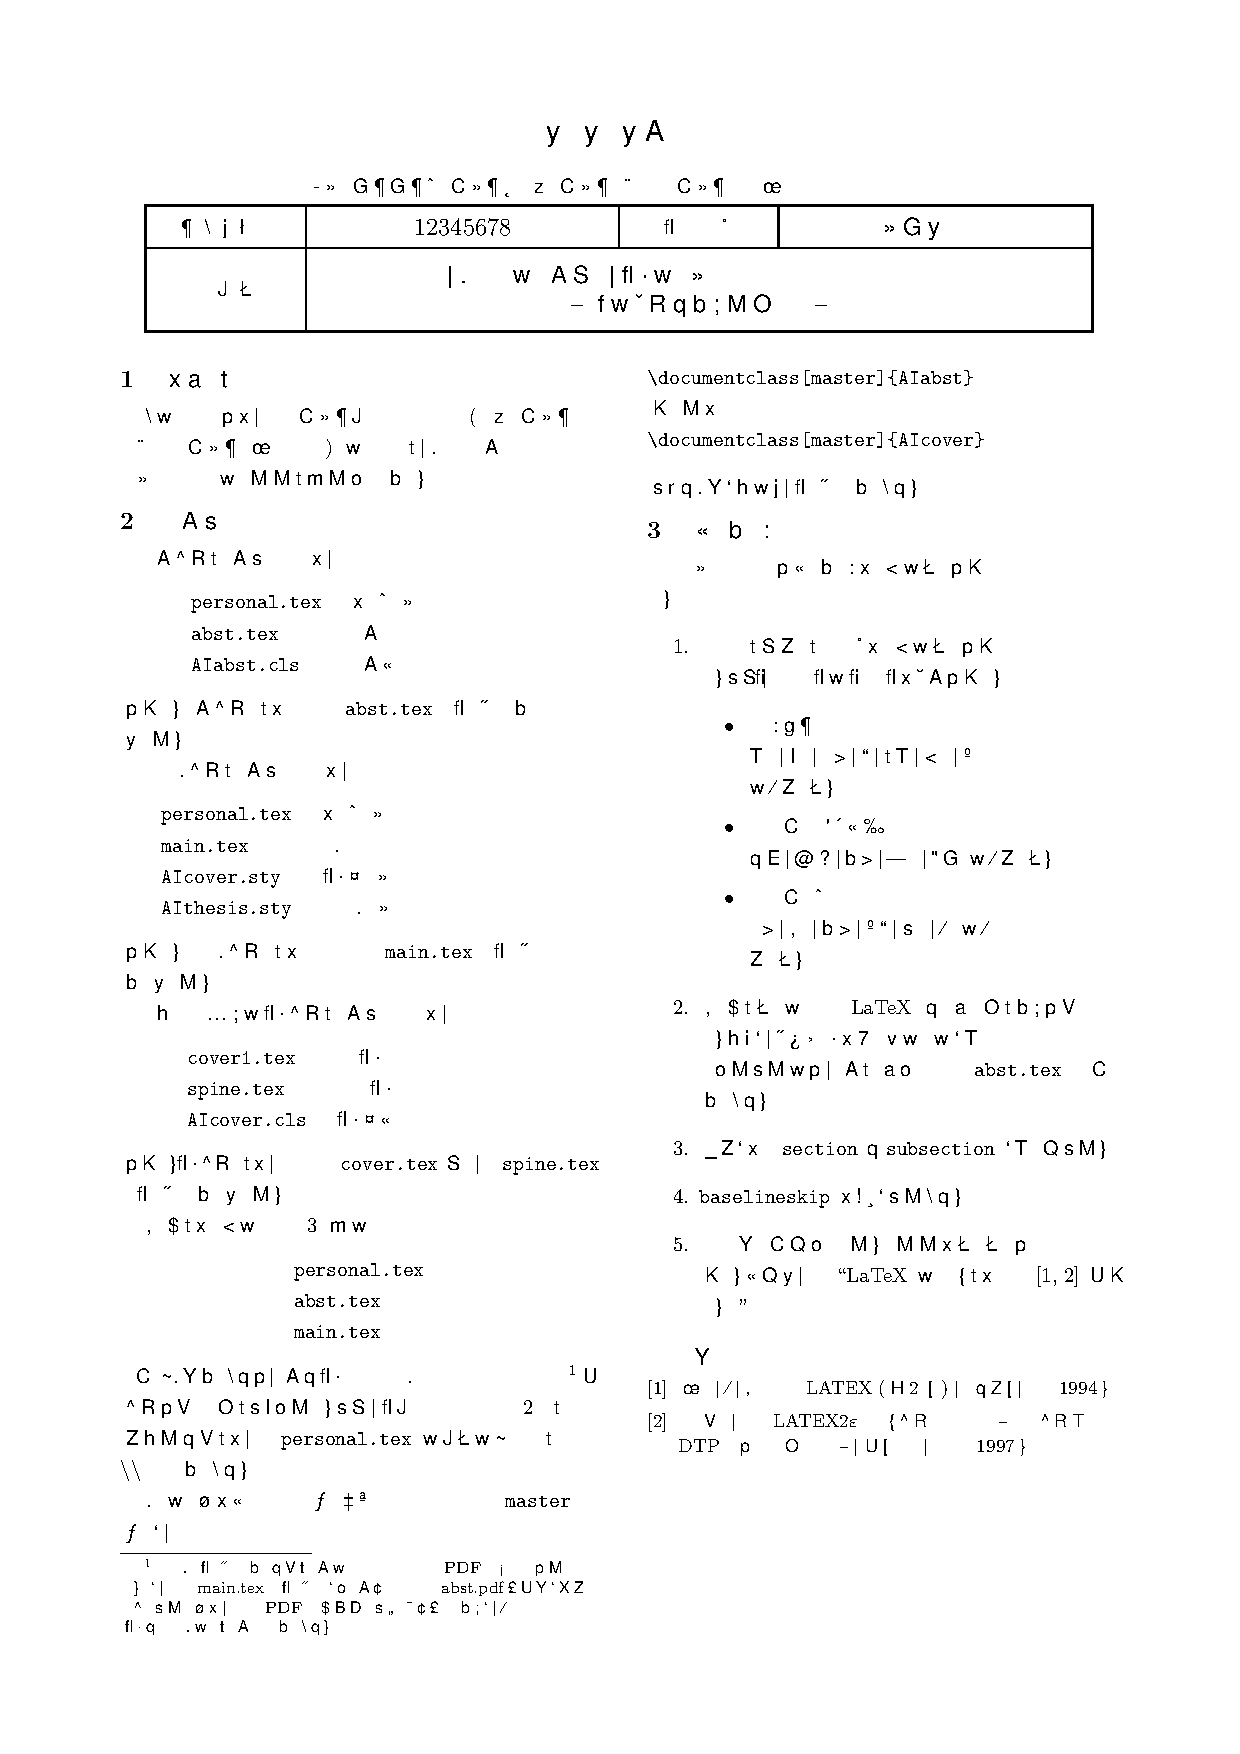
\includegraphics[width=21.0cm]{abst.pdf}
\end{figure}

\restoregeometry

\pagestyle{plain}
% 目次
\pagenumbering{roman}	%目次のページ番号(ローマ字)
\tableofcontents 		%目次作成
\newpage
\pagenumbering{arabic} 	%本編ページ番号

% Chapter1 : はじめに
\chapter{はじめに}
ここに「はじめに」を書く.

\section{論文の書式}
論文は,A4 版で,コピー用紙程度の上質紙に印字すること. 
書式は,過去の修士論文, 卒業論文等を参考にし,指導教員の指示を仰ぐこと. 
% この文書自体も通常の論文の形式({\tt bachelor.sty\/})に従っている.
%
\subsection{使用言語}
論文を記述するのに使用する言語は,日本語または英語とする.
%
\subsection{ページのレイアウト}
製本その他読みやすさ等を考慮して,マージンは大きめにとること.

\vspace*{3mm}
\hspace*{10mm}
\begin{tabular}{ll}
上マージン & 25mm 程度 \\
下マージン & 30mm 程度 (ページ番号もマージン内に含む) \\
左マージン & 35mm 程度 (製本の都合上 30mm 以上は必要) \\
右マージン & 25mm 程度 \\
\end{tabular}

\subsection{文字の大きさ}
読みやすさ等を考慮して,極端に小さい文字や大きな文字はさけ, 行間は十分にあけること. 
文字サイズ 11-12pt, 1ページ 30 行で日本語の場合は 1 行あたり 40 文字程度が目安となる. 

\subsection{製本方法}
提出する論文は学科事務室で配布するバインダを用いて製本する.
(バインダは,修士論文の場合は提出前に事前に,卒業論文の場合は卒業論文概要提出の際に受け取ること.)
綴じ穴は製本の都合上 2 穴,穴の位置は紙の端から 12mm とする. 

バインダーの表紙および背に,{\tt cover.tex\/}および{\tt spine.tex\/}を用いて作成した表紙,背表紙を貼り付けること. 

\subsection{提出について}
提出についての詳細は
修士論文は {\tt Mschedule.pdf},
卒業論文は {\tt Bschedule.pdf} を参照のこと.

\newpage

\end{document}

